\begin{frame}[allowframebreaks]{Conventions de représentation}
\textbf{\textit{Adjacent List Stucture}}\\
\begin{multicols}{2}
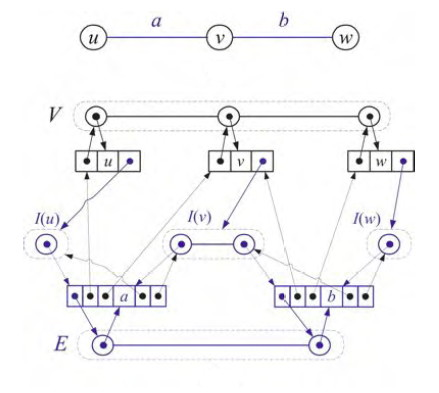
\includegraphics[scale=0.35]{images/schema.jpg}\\
\textbf{Objet noeud} : \begin{itemize}
\item Référence vers une liste chainée contenant des références vers les arêtes sortantes du noeud
\item Entier \textit{incounter} contenant le nombre d'arêtes entrantes au noeud\\
\end{itemize}

\textbf{Objet arête} : \begin{itemize}
\item Référence vers le noeud dont l'arête est la destination
\end{itemize}
\end{multicols}

\newpage
Avantages : \\
\begin{itemize}
\item \textbf{Facilité d'implémentation}
\item \textbf{Complexité} de l'algorithme en $\mathcal{O}(n+m)$ avec $n$ le nombre de noeuds et $m$ le nombre d'arêtes. C'est le meilleur choix possible car toutes les arêtes et tous les noeuds sont parcourus dans le pire des cas. De plus, la complexité est meilleure par rapport à
\begin{itemize}
\item l'\textit{edgelist structure} : \textit{IncidentEdges} en $\mathcal{O}(m)$
\item l'\textit{adjacency matrix structure} : \textit{IncidentEdges} en $\mathcal{O}(n)$
\end{itemize}
En effet, la complexité de \textit{IncidentEdges} est dans notre cas de $\mathcal{O}(1)$
\end{itemize}
\end{frame}
